\documentclass{standalone}
\usepackage{tikz}

\usetikzlibrary{intersections}


\begin{document}

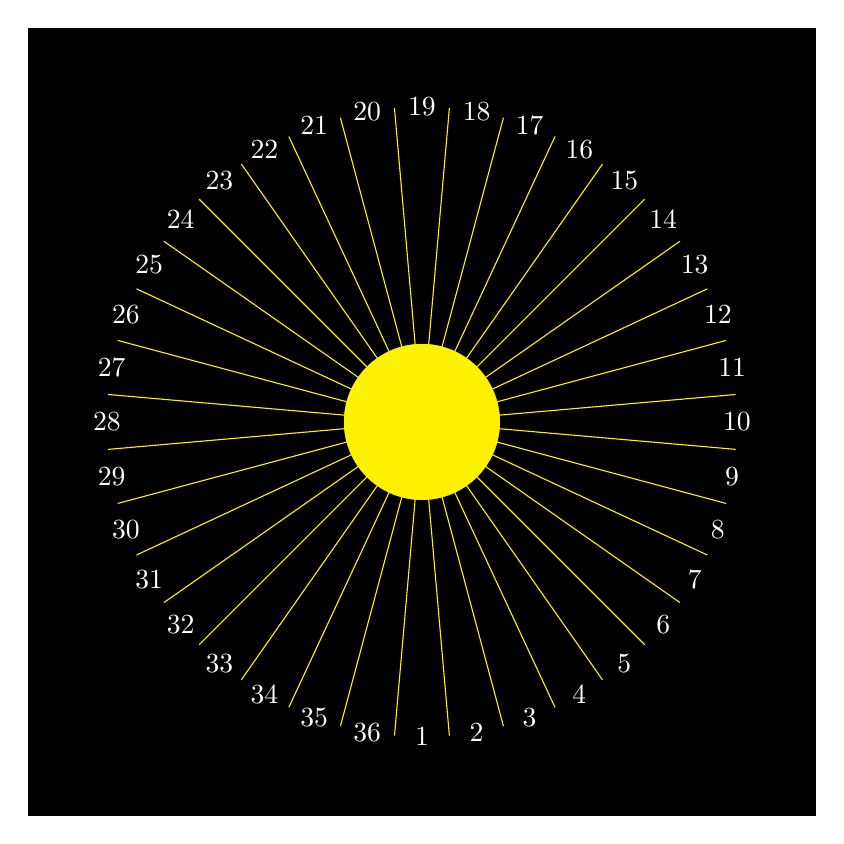
\begin{tikzpicture}
  \draw[fill=black,black] (-5,-5) rectangle (5,5);
  \draw[fill=yellow] (0,0) circle [radius=1cm];

  \foreach \x in {-95,-85,...,260} {
    \draw[thin,yellow] (0,0) -- (\x:4);
  }

  \foreach[count=\i] \x in {-90,-80,...,260} {
    \node[white] at (\x:4) {\i};
  }
\end{tikzpicture}

\end{document}